\section{Introduction}
\label{intro}


\newcommand{\xidx}{i}
\newcommand{\yidx}{j}
\newcommand{\xw}[1]{w_{#1}}
\newcommand{\yw}[1]{w'_{#1}}




\begin{center}$\vdots$\end{center}

As a motivating example, we consider the Simplified Arbiter problem.
Two processes $x$ and $y$ are scheduled to run $|x|$ and $|y|$ time slots,
respectively. Execution starts at $t=0$, and the length of each time slot is
one time unit. The cost for scheduling the slots $[i..p)$ of $x$ at $t=i+j$
is given by $\xw{ipj}$, and the cost for schedulting the slots $[j..q)$ of $y$
also at $t=i+j$ is given by $\yw{jqi}$.



The optimal cost for scheduling the first $i$ slots of $x$ and the first $j$ slots
of $y$ is given by the recurrence:

\begin{equation}
\renewcommand\arraystretch{1.5}
\begin{array}{l@{}l}
	G_{ij} ~=~  &
	\begin{cases}
		0                        & i=j=0 \\
		\yw{0j0}                  & i=0, j>0 \\
		\xw{0i0}                 & i>0, j=0 \\
		\begin{array}{@{}l@{~}l}
		  \min\langle & \underset{0\leq q<j}\min ~ G_{iq} + \yw{qji}, \\
		              & \underset{0\leq p<i}\min ~ G_{pj} + \xw{pij}~\rangle
		\end{array}              & i,j>0
	\end{cases}
\end{array}
\label{intro:gap spec}
\end{equation}
\smallskip\noindent
By way of intuition, the seconc case corresponds to the case when all the 
time has been allocated to $y$, so $i=0$ and the cost will be 
$\yw{0j0}$ by definition, and similarly for the third case. In the fourth case,
either the schedule ends with time allocated to $x$, in which case $x$ was allocated
time from 


So that the cost for the entire schedule is $G_{|x||y|}$.

\medskip
With standard dynamic programming, this recurrence can be computed
with an iterative program, by understanding the dependency pattern:
each value $G_{ij}$ is computed from other values $G_{i'j'}$ with lower
indexes, $i'<i$, ~$j'<j$. Therefore, considering $G$ as a two-dimensional
array, it can be filled in a single pass from left to right and from top
to bottom.

\newcommand\FORLINE[1]{\STATE\algorithmicfor~{#1} \algorithmicdo~}

\begin{algorithm}
\renewcommand\arraystretch{1.3}
\begin{algorithmic}
  \STATE $G_{00} := 0$
  \FORLINE{$j=1..|y|$}  $G_{0j} := w_{0j0}$  
  \FOR{$i=1..|x|$}
    \STATE $G_{i0} := w'_{i00}$
    \FOR{$j=1..|y|$}
      \STATE $G_{ij} :=
        \begin{array}[t]{@{}l@{~}l} 
          \min\langle & \underset{0\leq q<j}\min ~ G_{iq} + w_{qji}, \\
                      & \underset{0\leq p<i}\min ~ G_{pj} + w'_{pij}~\rangle 
        \end{array}$
    \ENDFOR
  \ENDFOR
\end{algorithmic}
\end{algorithm}

The same intuition underlies the divide-and-conquer approach for making
a parallel version of the same computation. The array $G$ is partitioned into
quadrants and dependencies are observed at the level of quadrants. The same reasoning
has to be repeated at a coarser level;
so, say the quadrants are labeled 1, 2, 3, and 4, then the computations of 2 and 3 depend on 1,
and the computation of 4 depends on 2 and 3 (\Cref{intro:quadrants}).

\newcommand\qbox[1]{\fbox{\scriptsize#1}}

\begin{figure}[b]
\quad
$\renewcommand\arraystretch{2}G ~=~
 \begin{array}{|@{\quad}c@{\quad}|@{\quad}c@{\quad}|} \hline 1 & 2 \\[1mm] \hline 3 & 4 \\[1mm] \hline\end{array}$
\qquad
$\begin{array}{l}\qbox1 \rightsquigarrow \qbox2 \\ 
\qbox1 \rightsquigarrow \qbox3 \\ \qbox2\rightsquigarrow \qbox4 \\ \qbox3 \rightsquigarrow \qbox4\end{array}$
\caption{\label{intro:quadrants}
  Top-level data dependencies.}
\end{figure}

\medskip
The algorithm designer then writes the following pseudo-code:

\begin{algorithmic}[1]
  \STATE Compute \qbox1 (using only input data $w,w'$).
  \STATE Compute \qbox2 using data from \qbox1.
  \STATE Compute \qbox3 using data from \qbox1.
  \STATE Compute \qbox4 using data from \qbox2 and \qbox3.
\end{algorithmic}

We say that the computation is \newterm{stratified},
in the sense that information flows only in one direction. It can be depicted as
a sequence of steps, each of which reads some regions from the array (possibly none)
and writes into a target region. It can be viewed as a chain, like the one in
\Cref{intro:chain}.

\begin{figure}
\includegraphics[width=.47\textwidth]{img/gap-stratify1}
\caption[caption]{\label{intro:chain}
  Stratified computation for Simplified Gap. \\[.2em]
  Thick borders indicate the region that is read at each step.}
\end{figure}

At this point it can be noticed that step 1 is equivalent to the original
algorithm when given as input the prefixes of $x$ and $y$ whose length correspond to the
height and width of \qbox1.

With the other three steps, however, things are not so simple:
each of them is required to process some data in addition to the input.
For example, step 2 is required to read values from \qbox1, due to the expression
$G_{iq}$ (where $\scriptstyle 0\leq q<j$).
In order to reason more formally, we define $J$ and $K$ the index sets of the rows
and columns, respectively; $J_0$, $J_1$ for the top and bottom row indexes, respectively;
and $K_0$, $K_1$ for the left and right column indexes (\Cref{intro:slice G}).
The specifications for step 2 then take the following form:

\begin{figure}
\[
\renewcommand\arraystretch{2}
\begin{array}{c|c|c|c|}
  \multicolumn{2}{c}{} & \multicolumn{2}{c}{K} \\ \cline{3-4}
  \multicolumn{2}{c}{} & \multicolumn{1}{c}{K_0}  & \multicolumn{1}{c}{K_1}\\ \cline{3-4}
  \multirow{2}{*}{$J$} & J_0 & 1 & 2 \\ \cline{3-4}
    & J_1 & 3 & 4 \\ \cline{3-4}
\end{array}
\]
\caption{\label{intro:slice G}
  Addressing quadrants in a two-dimensional array.}
\end{figure}

\makeatletter
\newcommand{\LeftEqNo}{\let\veqno\@@leqno}
\makeatother

\begin{equation}\LeftEqNo
\renewcommand\arraystretch{1.5}
\begin{array}{l@{}l}
	G_{\,(i : J_0)\,(j : K_1)} ~=~  \\
	\qquad
	\begin{cases}
		0                        & i=j=0 \\
		w_{0j}                   & i=0, j>0 \\
		w'_{i0}                  & i>0, j=0 \\
		\begin{array}{@{}l@{~}l}
		  \min\langle & \underset{0\leq (q:K) <j}\min ~ G_{iq} + w_{qj}, \\
		              & \underset{0\leq (p:J_0) <i}\min ~ G_{pj} + w'_{pi}~\rangle
		\end{array}              & i,j>0
	\end{cases}
\end{array}
\end{equation}

\medskip
Type annotations have been placed on $i$, $j$, $p$, and $q$ to define the regions
over which they range. $i:J_0, j:K_1$ means that the element $G_{ij}$
is always in \qbox2. Similarly, $G_{pj}$ is also in \qbox2. $G_{iq}$ is either in
\qbox1 or in \qbox2.

\begin{figure}
\quad
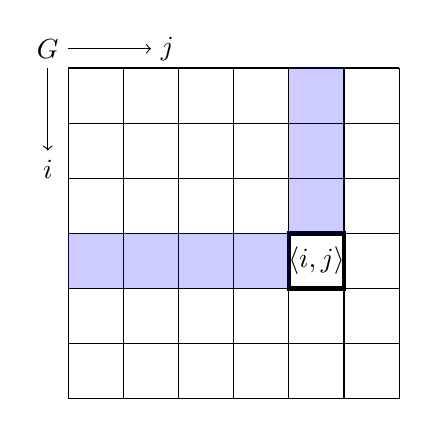
\begin{tikzpicture}[x=7mm,y=7mm,baseline=(center)]
  \coordinate(center) at (3,3);
  \draw[step=1] (0,0) grid (6,6);
  \draw[ultra thick] (4,2) rectangle +(1,1);
  \node at (4.5,2.5) {$\langle i,j\rangle$};
  \fill[blue,opacity=0.2] (0,2) rectangle (4,3);
  \fill[blue,opacity=0.2] (4,3) rectangle (5,6);
  \node[anchor=south east](G) at (0,6) {$G$};
  \draw[->] (G.east) -- +(1.5,0) node[anchor=west] {$j$};
  \draw[->] (G.south) -- +(0,-1.5) node[anchor=north] {$i$};
\end{tikzpicture}
\qquad

\begin{tikzpicture}[x=3mm,y=3mm,baseline=(squig)]
  \draw[fill=blue, fill opacity=0.2] (0,0) rectangle +(1,1);
  \draw[ultra thick] (2.6,0) rectangle +(1,1);
  \node(squig) at (1.8,.5) {$\rightsquigarrow$};
\end{tikzpicture}
\caption{\label{intro:gap dependency matrix}
  Cell-level data dependencies.}
\end{figure}

To address the situation, the algorithm designer would like to separate the parts
of the computation that read from \qbox1 from the parts that read from \qbox2.
This can be achieved here by splitting the $\min_{0\leq(q:K)<j}$ into two
ranges, according to the region in which $G_iq$ resides.

\begin{equation}\LeftEqNo
\renewcommand\arraystretch{1.5}
\begin{array}{l@{}l}
	G_{\,(i :: J_0)\,(j :: K_1)} ~=~  \\
	\qquad
	\begin{cases}
		0                        & i=j=0 \\
		w_{0j}                   & i=0, j>0 \\
		w'_{i0}                  & i>0, j=0 \\
		\begin{array}{@{}l@{~}l}
		  \min\langle & \underset{(q:K_0)}\min ~ G_{iq} + w_{qj}, \\
		              & \underset{(q:K_1) <j}\min ~ G_{iq} + w_{qj}, \\
		              & \underset{0\leq (p:J_0) <i}\min ~ G_{pj} + w'_{pi}~\rangle
		\end{array}              & i,j>0
	\end{cases}
\end{array}
\end{equation}

The path becomes clear: compute $\min_{(q:K_0)} ~ G_{iq} + w_{qj}$ first, for all $i$, $j$
in \qbox2. Then use the results to compute $G_{ij}$.

\begin{equation}\LeftEqNo
\renewcommand\arraystretch{1.5}
\begin{array}{l@{}l}
	G_{\,(i : J_0)\,(j : K_1)} ~=~  \\
	\qquad
	\textrm{let}~\psi_{ij} = \underset{(q::K_0)}\min ~ G_{iq} + w_{qj} \\
	\qquad\textrm{in} \\
	\qquad
	\begin{cases}
		0                        & i=j=0 \\
		w_{0j}                   & i=0, j>0 \\
		w'_{i0}                  & i>0, j=0 \\
		\begin{array}{@{}l@{~}l}
		  \min\langle & \psi_{ij}, \\
		              & \underset{(q:K_1) <j}\min ~ G_{iq} + w_{qj}, \\
		              & \underset{0\leq (p:J_0) <i}\min ~ G_{pj} + w'_{pi}~\rangle
		\end{array}              & i,j>0
	\end{cases}
\end{array}
\label{intro:let in 2}
\end{equation}

\medskip
The second part in \eqref{intro:let in 2} starts to look similar to \eqref{intro:gap spec}:
in particular, the types of $p$ and $q$ are the same as those of $i$ and $j$.
In fact, if we set $\psi_{ij}=\infty$, we get \eqref{intro:gap spec} as a special case,
only with $J_0$ and $K_1$ instead of $J$ and $K$.
It therefore makes sense to write a version that generalizes both.

\begin{equation}\LeftEqNo
\renewcommand\arraystretch{1.5}
\begin{array}{l}
	A^{^{JK}}_{\,\psi\, i\, j} ~=~  \\
	\qquad
	\begin{cases}
		0                        & i=j=0 \\
		w_{0j}                   & i=0, j>0 \\
		w'_{i0}                  & i>0, j=0 \\
		\begin{array}{@{}l@{~}l}
		  \min\langle & \psi_{ij}, \\
		              & \underset{(q:K)<j}\min ~ A^{^{JK}}_{\psi iq} + w_{qj}, \\
		              & \underset{(p:J)<i}\min ~ A^{^{JK}}_{\psi pj} + w'_{pi}~\rangle
		\end{array}              & i,j>0
	\end{cases}
\end{array}
\label{intro:gap phase A}
\end{equation}

\medskip
And we can now rewrite \eqref{intro:gap spec} and \eqref{intro:let in 2} as
%
\begin{equation}
	G_{ij} ~=~ A^{^{JK}}_{\,(\infty^{J\times K})\,(i:J)\,(j:K)}
\end{equation}
%
\begin{equation}
\renewcommand\arraystretch{1.3}
\begin{array}{l@{}l}
	G_{\,(i : J_0)\,(j : K_1)} ~=~ 
	& \textrm{let}~\psi_{ij} = \underset{(q:K_0)}\min ~ G_{iq} + w_{qj} \\
	& \textrm{in}~A^{^{J_0K_1}}_{\,\psi ij}
\end{array}	
\label{intro:let in 2 using A}
\end{equation}

\newcommand\otherwise{\textrm{\small otherwise}}

\medskip
It takes a bit more insight to notice that \eqref{intro:let in 2 using A} can be further
generalized into:
%
\begin{equation}\LeftEqNo
\renewcommand\arraystretch{1.5}
\begin{array}{l@{}l}
	A^{^{JK}}_{\,\psi\,(i : J_0)\,(j : K_1)} ~=~ \\
	\qquad
	\textrm{let}~\psi'_{ij} = \begin{cases}
	  \begin{array}{@{}l@{}l@{}}\min\langle & \psi_{ij}, \\ & \!\underset{(q:K_0)}\min ~ A^{^{J_0K_0}}_{\,\psi iq} + w_{qj}\rangle\end{array} & \langle i,j\rangle\mbox{ in }\qbox2 \\
	  \psi_{ij} & \otherwise
	\end{cases} \\
	\qquad\textrm{in}~
	A^{^{J_0K_1}}_{\,\psi' ij}
\end{array}
\label{intro:let in A 2}
\end{equation}

That is the core of the divide and conquer method: representing the output as a combination
of smaller instances of the problem, or sub-problems, yielding a solution that is essentially
a recursive routine, or a set of mutually recursive routines. 
Once all the pieces fit together, it is possible to cut the space into arbitrarily small pieces,
that fit nicely in each core's local cache. This greately increases performance, as demonstrated
by~\citneeded{perhaps include a table with exact figures}. 
\todo{Find a way to make this statement earlier}

\medskip
Similarly for \qbox3 and \qbox4:
%
\begin{equation}\LeftEqNo
\renewcommand\arraystretch{1.5}
\begin{array}{l@{}l}
	A^{^{JK}}_{\,\psi\,(i : J_1)\,(j : K_0)} ~=~ \\
	\qquad
	\textrm{let}~\psi'_{ij} = \begin{cases} 
	  \begin{array}{@{}l@{}l@{}}\min\langle & \psi_{ij}, \\ & \!\underset{(p:J_0)}\min ~ A^{^{J_0K_0}}_{\,\psi pj} + w'_{pi}\rangle \end{array} & \langle i,j\rangle\mbox{ in }\qbox3 \\
	  \psi_{ij} & \otherwise \\
	\end{cases} \\
	\qquad\textrm{in}~
	A^{^{J_1K_0}}_{\,\psi' ij}
\end{array}
\label{intro:let in A 3}
\end{equation}

\begin{equation}\LeftEqNo
\renewcommand\arraystretch{1.5}
\begin{array}{l@{}l}
	A^{^{JK}}_{\,\psi\,(i : J_1)\,(j : K_1)} ~=~ \\
	\qquad
	\textrm{let}~\psi'_{ij} = \begin{cases} 
	  \begin{array}{@{}l@{}l@{}}\min\langle & \psi_{ij}, \\
         & \!\underset{(q:K_0)}\min ~ A^{^{J_1K_0}}_{\,\psi iq} + w'_{qj}\rangle \\
         & \!\underset{(p:J_0)}\min ~ A^{^{J_0K_1}}_{\,\psi pj} + w'_{pi}\rangle \end{array} & \langle i,j\rangle\mbox{ in }\qbox4 \\
	  \psi_{ij} & \otherwise \\
	\end{cases} \\
	\qquad\textrm{in}~
	A^{^{J_1K_0}}_{\,\psi' ij}
\end{array}
\label{intro:let in A 4}
\end{equation}

Evidently there are some common sub-expressions. Defining
\begin{equation}
\renewcommand\arraystretch{1.3}
\begin{array}{l@{}l@{}l}
	B^{^{JK_0K_1}}_{\,\psi\,(i : J)\,(j : K_1)} ~=~ &
	  \min\langle & \psi_{ij}, \\ 
	&  & \!\underset{(q:K_0)}\min ~ \psi_{iq} + w_{qj}\rangle \\[.8em]
	C^{^{J_0J_1K}}_{\,\psi\,(i : J_1)\,(j : K)} ~=~ &
	  \min\langle & \psi_{ij}, \\ 
	&  & \!\underset{(p:J_0)}\min ~ \psi_{pj} + w'_{pi}\rangle 
\end{array}
\end{equation}

We can write \eqref{intro:let in A 2}, \eqref{intro:let in A 3}, \eqref{intro:let in A 4} as ---

\begin{equation}\LeftEqNo
\renewcommand\arraystretch{1.5}
\begin{array}{l@{}l}
	A^{^{JK}}_{\,\psi\,(i : J_0)\,(j : K_1)} ~=~ \\
	\qquad
	\textrm{let}~\psi'_{ij} = \begin{cases}
	  B^{^{J_0K_0K_1}}_{\psi ij} & \langle i,j\rangle\mbox{ in }\qbox2 \\
	  \psi_{ij} & \otherwise
	\end{cases} \\
	\qquad\textrm{in}~
	A^{^{J_0K_1}}_{\,\psi' ij}
\end{array}
\label{intro:let in A 2 using B}
\end{equation}

\begin{equation}\LeftEqNo
\renewcommand\arraystretch{1.5}
\begin{array}{l@{}l}
	A^{^{JK}}_{\,\psi\,(i : J_1)\,(j : K_0)} ~=~ \\
	\qquad
	\textrm{let}~\psi'_{ij} = \begin{cases}
	  C^{^{J_0J_1K_0}}_{\psi ij} & \langle i,j\rangle\mbox{ in }\qbox3 \\
	  \psi_{ij} & \otherwise
	\end{cases} \\
	\qquad\textrm{in}~
	A^{^{J_1K_0}}_{\,\psi' ij}
\end{array}
\label{intro:let in A 2 using B}
\end{equation}

\begin{equation}\LeftEqNo
\renewcommand\arraystretch{1.5}
\begin{array}{l@{}l}
	\lspan2{A^{^{JK}}_{\,\psi\,(i : J_1)\,(j : K_1)} ~=~} \\
	\qquad
	\textrm{let}~ & \psi'_{ij} = \begin{cases}
	  B^{^{J_1K_0K_1}}_{\psi ij} & \langle i,j\rangle\mbox{ in }\qbox4 \\
	  \psi_{ij} & \otherwise
	\end{cases} \\[1.2em]
	& \psi''_{ij} = \begin{cases}
	  C^{^{J_0J_1K_1}}_{\psi' ij} & \langle i,j\rangle\mbox{ in }\qbox4 \\
	  \psi_{ij} & \otherwise
	\end{cases} \\
	\lspan2{
	\qquad\textrm{in}~A^{^{J_1K_0}}_{\,\psi'' ij}
	}
\end{array}
\label{intro:let in A 2 using B}
\end{equation}

$B$ and $C$ are two more sub-problems that have to be addressed using the same slicing technique.
Seems we have completed one task but created two? --- Fortunately, $B$ and $C$ are much simpler instances\todo{for once, they are not recursive}
and are quite easy to develop.\todo{show this? Forget about this paragraph??}


\begin{center}$\vdots$
\end{center}


\begin{figure*}
\resizebox{\textwidth}{!}{
\begin{tikzpicture}
	\begin{axis}[
	    title=Parenthesis,
	    ymode=log,
		xlabel=$n$,
		ylabel=Time ({\it s}),
		scaled x ticks=false, %{real:1000}
		log basis y=2, ymajorgrids=true]
	\addplot[color=blue!50!white,ultra thick,mark=*,smooth] table[x=n/Time(s),y=COZ] {data/plot1.dat}
	  [yshift=-8pt] node[pos=0] {CO};
	\addplot[color=red!70!white,ultra thick,mark=*,smooth] table[x=n/Time(s),y=Tiled/Par] {data/plot1.dat}
	  [yshift=-10pt] node[pos=0] {PluTo};
	\end{axis}
\end{tikzpicture}
\begin{tikzpicture}
	\begin{axis}[
	    title=Gap,
	    ymode=log,
		xlabel=$n$,
		scaled x ticks=false, %{real:1000}
		log basis y=2, ymajorgrids=true]
	\addplot[color=blue!50!white,ultra thick,mark=*,smooth] table[x=n/Time(s),y=COZ] {data/plot2.dat}
	  [yshift=-8pt] node[pos=0] {CO};
	\addplot[color=red!70!white,ultra thick,mark=*,smooth] table[x=n/Time(s),y=Tiled/Par] {data/plot2.dat}
	  [yshift=-8pt] node[pos=0] {PoCC};
	\end{axis}
\end{tikzpicture}
\begin{tikzpicture}
	\begin{axis}[
	    title=Floyd-Warshall,
	    ymode=log,
		xlabel=$n$,
		scaled x ticks=false, %{real:1000}
		log basis y=2, ymajorgrids=true]
	\addplot[color=blue!50!white,ultra thick,mark=*,smooth] table[x=n/Time(s),y=COZ] {data/plot3.dat}
	  [yshift=-8pt] node[pos=0] {CO};
	\addplot[color=red!70!white,ultra thick,mark=*,smooth] table[x=n/Time(s),y=Tiled/Par] {data/plot3.dat}
	  [yshift=-8pt] node[pos=0] {PoCC};
	\end{axis}
\end{tikzpicture}
}
\caption{\label{intro:coz speedup}
  Comparison of the the best performance obtained using polyhedral compilers 
  (PluTo\,\cite{HPC10/Pouchet}, PoCC\,\cite{PLDI08/Bondhugula})
  for parallelization, vs. manually crafted recursive divide-and-conquer implementations (CO).}
\end{figure*}

\subsection{Main Contributions}

\begin{enumerate}
  \item We develop a small set of formal tactics that can be used to transform a class of recurrence
  specifications, written in a simple functional language, 
  into equivalent divide-and-conquer programs, that admit parallel cache-local
  implementations, in a principled, systematic manner.
  \item We prove that these tactics are semantics-preserving, assuming some side conditions are met
  at the point when the tactic is applied.
  \item We show that the side conditions can be effectively translated into first-order closed
  formulas, and verified automatically by SMT solvers.
\end{enumerate}

